 \documentclass[12pt]{report}
% ---------------------- Required Packages ----------------------
\usepackage{Styles/GUB}               % Custom style
\usepackage[utf8]{inputenc}          % For UTF-8 encoding
\usepackage[english]{babel}          % English language
\usepackage{graphicx}                % Graphics inclusion
\usepackage{caption}
\usepackage{subcaption}             % Subfigures
\usepackage{float}                  % For forcing table/figure position
\usepackage{amsmath, amssymb, amsfonts} % Math packages
\usepackage{bm}                     % Bold math
\usepackage{mathptmx}               % Times font
\usepackage{siunitx}                % SI units
\usepackage{array}                  % Extended tables
\usepackage{longtable}
\usepackage{adjustbox}
\usepackage{booktabs}               % Better tables
\usepackage{multirow}
\usepackage{tabularx}               % Tables with flexible columns
\usepackage[table]{xcolor}
\usepackage{url}                    % Format URLs
\usepackage{xcolor}                 % Colored text


% Please add the following required packages to your document preamble:
% \usepackage{multirow}
\usepackage[table,xcdraw]{xcolor}
%\usepackage{colortbl}
\usepackage{pdflscape}
\usepackage[normalem]{ulem}
\useunder{\uline}{\ul}{}
\usepackage{lipsum}                 % Dummy text
\usepackage{fancyhdr}               % Fancy headers
\usepackage{epstopdf}               % EPS support
\usepackage{enumerate}              % Custom enumeration
\usepackage[utf8]{inputenc}
\usepackage{adjustbox}              % Box adjustment
\usepackage[margin=1in]{geometry}   % Overall page layout
\usepackage{hyperref}
\hypersetup{
    colorlinks=true,
    linkcolor=magenta,
    citecolor=magenta,
    urlcolor=magenta,
    filecolor=magenta
}

\usepackage[a4paper, left=1.5in, right=1in, bottom=1.3in]{geometry}

\usepackage{ragged2e}
\usepackage[utf8]{inputenc}

\hypersetup{colorlinks=true, linkcolor=black, filecolor=magenta, urlcolor=cyan}
\usepackage[nottoc,notlof,notlot]{tocbibind} 
\usepackage{pifont}                 % Special symbols
\usepackage{lscape}                 % Landscape tables
\usepackage{mwe}                    % Example images
\usepackage{nomencl}                % List of symbols
\usepackage{algorithm2e}            % Algorithms
\usepackage{epsfig}                 % EPS figures (if needed)
\usepackage{listings}

% \usepackage{tikz}
% \usetikzlibrary{arrows,positioning}
% \usetikzlibrary{positioning}


\lstset{
    basicstyle=\ttfamily\small,
    keywordstyle=\color{blue},
    commentstyle=\color{gray},
    stringstyle=\color{purple},
    showstringspaces=false,
    breaklines=true,
    frame=single
}


\lstdefinestyle{tree}{
  basicstyle=\ttfamily\small,
  backgroundcolor=\color{gray!5},
  frame=single,
  breaklines=true,
  showstringspaces=false
}

\lstdefinestyle{bash}{
    backgroundcolor=\color{gray!10},
    basicstyle=\ttfamily\footnotesize,
    frame=single,
    breaklines=true,
    showstringspaces=false,
    language=bash
}

% ---------------------- Algorithm2e Settings ----------------------
\SetKwInput{KwInput}{Input}
\SetKwInput{KwOutput}{Output}
\newcommand\mycommfont[1]{\footnotesize\ttfamily\textcolor{blue}{#1}}
\SetCommentSty{mycommfont}
\SetAlgoNlRelativeSize{0}

% ---------------------- General Settings ----------------------
\renewcommand{\baselinestretch}{1.5}
\pagestyle{plain}
\renewcommand{\labelenumi}{\alph{enumi}.}

% ---------------------- Column Types for Tables ----------------------
\newcolumntype{C}{>{\raggedright\arraybackslash}p{18em}}
\newcolumntype{D}{>{\raggedleft\arraybackslash}p{15.5em}}

\begin{document}

% ---------------------- Front Matter ----------------------
\begin{titlepage}
\begin{center}

% YOU MUST ENSURE THAT THE GUB LOGO AND COMPANY LOGO ARE PROPERLY ALIGNED

% --- Logos Row ---
% \vspace{0.0cm}

\begin{figure}[h!]
    \centering
    \begin{subfigure}[b]{0.3\textwidth}
        \centering
        
\includegraphics[width=0.8\textwidth]{figures/GUBLogoNew.png}
    \end{subfigure}
    \hfill
    \begin{subfigure}[b]{0.3\textwidth}
        \centering
        
\includegraphics[width=0.7\textwidth]{figures/dummy_600x400_000000_bfc635_company-logo.png}
    \end{subfigure}
\end{figure}

\vspace{0.6cm}

% --- University Name ---
{\Large \textbf{GREEN UNIVERSITY OF BANGLADESH}}

\vspace{0.6cm}

% --- Title ---
\fontsize{12}{14}\selectfont
\textbf{Industrial Training}\\
\textbf{on}\\
\textbf{Report Title}

\vspace{0.8cm}

% --- Submitted by ---
\textbf{Submitted by}\\
Student Name – Student ID (e.g. M. A. Al Sami - 211902058)

\vspace{0.8cm}

% --- Submission Purpose ---
\begin{minipage}{1\textwidth}
\centering
\textit{An industrial training report submitted to the Department of Computer Science \& Engineering, for the partial fulfillment of the degree of Bachelor of Science in Computer Science \& Engineering}
\end{minipage}

\vspace{0.8cm}

% --- Supervisor Info ---
\textbf{Under the Supervision of}\\
Md. Solaiman Mia\\
Assistant Professor, Department of CSE

\vspace{0.8cm}

% --- Training Place Info ---
\textbf{Training Place}\\
Company Name\\
Company Address

\vspace{0.8cm}

% --- Details Table ---
\begin{tabular}{@{}ll}
\hspace{1.8cm}\textbf{Training Duration    :} & DD.MM.YYYY to DD.MM.YYYY \\
\hspace{1.8cm}\textbf{Industrial Supervisor      :} & Supervisor Name \\
% \hspace{1.8cm}\textbf{Academic Supervisor      :} & Supervisor Name \\
\hspace{1.8cm}\textbf{Report Submission Date          :} & 28.09.2026 \\
\end{tabular}

\vspace{0.8cm}

\thispagestyle{empty}
\vspace*{\fill}
\begin{center}
    {\Large \textbf{Summer 2026}}
\end{center}
\vspace*{\fill}

\end{center}
\end{titlepage}

\pagenumbering{roman}
\chapter*{\centering Declaration}
\addcontentsline{toc}{chapter}{Declaration}

Declaring this training report to be founded only on my own research results, I make it clear. References are made to research materials discovered by other researchers. This work has not been submitted for a degree before, either in full or in part.


\bigskip
\bigskip
\bigskip


\begin{tabular}{p{5cm}p{5cm}p{5cm}}
\centering
  % after \\: \hline or \cline{col1-col2} \cline{col3-col4} ...
     &  &   \\
     &  &   \\
     &  &   \\
 \rule{4cm}{1pt}
 \\
  Monalisa Bargman \\
  ID: 221902098

  
\end{tabular}
\chapter*{\centering Certificate}
\addcontentsline{toc}{chapter}{Certificate}

This is to certify that the industrial training report entitled \textit{Business Analysis and Digital Solution Design for Industrial Energy and IIoT Monitoring Systems} has been prepared and submitted by \textbf{Monalisa Bargman} in partial fulfillment of the requirements for the degree of Bachelor of Science in Computer Science and Engineering on 28.09.2026.

\bigskip
\bigskip
\bigskip
\bigskip

\noindent
\begin{tabular}{p{7cm} p{2cm} p{7cm}}
  \rule{6cm}{1pt} & & \rule{5cm}{1pt} \\
  Md. Solaiman Mia  & & Md. Mochaddec Hossain \\
  Green University of Bangladesh & & Active Green Energy Ltd. \\
\end{tabular}

\bigskip
\noindent
\begin{center}
    \vspace{0.5cm}
    \textit{Accepted and approved in partial fulfillment of the requirements for the degree\\
    Bachelor of Science in Computer Science and Engineering.}
    \vspace{0.5cm}
\end{center}

\noindent
\begin{tabular}{p{6cm} p{3cm} p{6cm}}
  &  &  \\
  &  &  \\
  \rule{6cm}{1pt} &  & \\
  Syed Ahsanul Kabir \\
  Chairman \\ \\
  &  &  \\
  \rule{5cm}{1pt} &  & \rule{5cm}{1pt} \\
  Board Member & & Board Member \\
\end{tabular}

% For this report template, we cordially acknowledge the contributions of:
% Md. Abdullah Al Sami (211902058), Department of CSE, Green University of Bangladesh,
% Dr. Muhammad Aminur Rahman, Former Chairperson and Associate Professor, Department of CSE, GUB,
% Md. Ataullha, Editor of the Internship Report Template and Lecturer, CSE, GUB,
% Professor Dr. Ahsan Habib Tareq, Chairperson, Department of CSE, GUB,
% Ms. Shamima Akter, Assistant Professor, CSE, GUB, Chair, Internship Coordination Board,
% Md. Zahidul Hasan, Member Internship Coordination Board,  Lecturer, CSE, GUB.

\chapter*{\centering Acknowledgments}
\addcontentsline{toc}{chapter}{Acknowledgments}

I would like to express my sincere gratitude to all those who supported and guided me throughout the industrial training period from \textbf{[Start Date]} until \textbf{[End Date]}. Their encouragement and assistance were invaluable, especially during times when I faced challenges.

I am thankful to my academic mentor, \textbf{[Academic Supervisor's Name and Designation]}, for providing consistent guidance and support during the training. Their feedback and suggestions helped me stay focused and improved the overall quality of my learning experience.

I am also grateful to the professionals at \textbf{[Company/Organization Name]} for their valuable insights, technical guidance, and for sharing their industry experience. Their support greatly enhanced my understanding of real-world practices, tools, and work culture.

Finally, I would like to thank \textbf{[Family, Friends, or Personal Support Acknowledgments]} for their constant encouragement, emotional support, and motivation, which played a vital role in helping me successfully complete the training.

\bigskip

\textcolor{blue}{\textbf{This internship report is inspired by a template originally designed for a `Software Quality Assurance` field internship. As a result, some figures may reflect that context. Students are advised to review the instructions carefully and replace or update the figures appropriately, ensuring alignment with their own internship experience while following the structure of the template.}}

% For this report template, we cordially acknowledge the contributions of:
% Md. Abdullah Al Sami (211902058), Department of CSE, Green University of Bangladesh,
% Dr. Muhammad Aminur Rahman, Former Chairperson and Associate Professor, Department of CSE, GUB,
% Md. Ataullha, Editor of the Internship Report Template and Lecturer, CSE, GUB,
% Professor Dr. Ahsan Habib Tareq, Chairperson, Department of CSE, GUB,
% Ms. Shamima Akter, Assistant Professor, CSE, GUB, Chair, Internship Coordination Board,
% Md. Zahidul Hasan, Member Internship Coordination Board,  Lecturer, CSE, GUB.
% \chapter*{\centering Abstract}
% \addcontentsline{toc}{chapter}{Abstract}
% \par \textbf{S}oftware \textbf{Q}uality \textbf{A}ssurance (SQA) testing is faced with issues of dynamic requirements, resource limitations and the complexity of system interactions. The industrial training program I went through with QA Harbor Limited proved to be a great experience offering much needed knowledge on how to tackle such challenges entirely through practical experience on the manual testing part as well as on the automation testing side. The main focus of the program lay in the application of a structured approach toward the SQA, in the sense of having tested a structured analysis, as well as structured planning, complete test case development, test execution, with tracking of defects and detailed reporting, ultimately aiming for the reliability, integrity, and usability of software and web application system. During my industrial training, I conducted software quality testing on two projects such as manual testing on \textbf{Bikroy.com}. I have used Playwright for automation testing, Apache JMeter for load testing and Postman with REST API for API testing through the QA Harbor website knowns as \textbf{Labsqajobs.com}. Functional testing, performance testing, and security testing, among others, were also covered with the training that taught some of the important methodologies of SQA. This immersive was my ticket to learning the skills and understanding how to thrive in contemporary software quality assurance positions in any renowned IT company.\\

\chapter*{\centering Abstract}
\addcontentsline{toc}{chapter}{Abstract}

\par
% Briefly introduce the training domain and main objective.
This report summarizes the industrial training experience carried out at \textbf{[Company/Organization Name]}, focusing on the practical application of concepts related to \textbf{[Domain or Field, e.g., Software Quality Assurance]}. The primary objective of the training was to gain hands-on experience and enhance professional skills in a real-world environment.

% Mention main tools, technologies, or frameworks used.
The training involved working with various tools and technologies such as \textbf{[List key tools, technologies, or frameworks]}, following industry-standard methodologies. 

% Describe key responsibilities or tasks performed.
Tasks included \textbf{[Describe major responsibilities or activities]}, allowing exploration of practical aspects of \textbf{[Mention specific areas like manual testing, API development, etc.]}.

% Highlight projects, skills developed, and teamwork.
Throughout the training, involvement in \textbf{[Mention projects or modules]} helped strengthen problem-solving skills and technical competencies. Collaborative work within a professional team contributed to improved communication and time management abilities.

% Conclude with learning outcomes and relevance.
This internship provided a comprehensive learning experience, bridging academic knowledge with industry practice, and prepared me for future professional roles in the field of \textbf{[Relevant field or industry]}.

\vspace{0.5cm}

\noindent\textbf{Keywords:} % Add 3-5 keywords related to your training here
[Keyword1, Keyword2, Keyword3, ...]


\tableofcontents
\newpage
\listoffigures
\addcontentsline{toc}{chapter}{List of Figures}
\newpage
\listoftables
\addcontentsline{toc}{chapter}{List of Tables}

% ---------------------- Main Matter ----------------------
\newpage
\pagenumbering{arabic}
\setcounter{page}{1}

\chapter{Introduction}

\par \textbf{Industrial Training} serves as an essential link between academic knowledge and professional work experience. It provides students with the opportunity to apply theoretical concepts learned in the classroom to practical, real-world situations within an organizational setting. This hands-on exposure helps students develop not only technical skills but also important soft skills such as communication, teamwork, and time management, which are vital for success in the professional environment.

\par The primary purpose of industrial training is to prepare students for the workforce by familiarizing them with workplace culture, industry practices, and operational procedures. It enables students to face real challenges, learn problem-solving techniques, and understand the expectations of a professional setting. By engaging in actual projects, interns can bridge the gap between academic theories and industrial applications.

\section{Problem Domain}

\par This industrial training report documents my experiences and learning outcomes during my internship at [Company Name]. During this period, I was involved in [briefly mention area of focus or department, e.g., Software Testing, Marketing, Mechanical Engineering]. As a trainee, I encountered various challenges such as [mention typical issues like unfamiliarity with company tools, adapting to professional workflows, or specific technical difficulties]. Support from supervisors and colleagues helped me overcome these challenges and successfully contribute to assigned tasks.

\section{Motivation of Training}

\par The motivation behind pursuing industrial training includes:

\begin{itemize}
    \item \textbf{Professional Development:} Gaining practical experience and developing relevant skills aligned with the industry.
    \item \textbf{Career Exploration:} Understanding different career paths and industry environments.
    \item \textbf{Application of Knowledge:} Applying academic theories in a practical setting to reinforce learning.
    \item \textbf{Skill Enhancement:} Improving technical, analytical, and interpersonal skills through real work exposure.
    \item \textbf{Adaptability:} Learning to work effectively within a dynamic and evolving workplace.
    \item \textbf{Networking:} Building professional relationships and receiving mentorship.
    \item \textbf{Career Foundation:} Preparing for future employment by gaining hands-on experience and industry insights.
\end{itemize}

\section{Objective of Training}

\par The objectives of this industrial training program are:

\begin{itemize}
    \item To gain practical experience in [mention relevant field, e.g., software quality assurance, marketing strategies].
    \item To develop problem-solving skills through participation in real projects.
    \item To understand and apply industry standards, tools, and best practices.
    \item To improve communication and collaboration skills by working with professionals.
    \item To familiarize myself with current technologies and workflows used in the industry.
    \item To contribute meaningfully to the organization’s goals through assigned tasks.
\end{itemize}

\section{Scope of Training}

\par The scope of this industrial training encompassed activities directly related to [mention specific field or department, e.g., software testing, mechanical design, marketing campaigns]. It included hands-on project work, participation in team meetings, and use of industry-standard tools. Areas outside the core project scope, such as unrelated departments or advanced research work, were not covered. This focus ensured concentrated skill development and meaningful contributions within the assigned domain.


\section{Identifying the Gap Between Academia and Industry}

\par There is often a notable gap between academic learning and industry requirements. Common causes include:

\begin{itemize}
    \item \textbf{Theoretical Knowledge vs Practical Application:} Academic curricula often focus on theory, with limited exposure to practical challenges and real-world constraints.
    \item \textbf{Limited Access to Industry Tools:} Students may not have hands-on experience with current technologies and software widely used in the industry.
    \item \textbf{Work Environment Dynamics:} Academic projects usually lack the collaborative and multidisciplinary teamwork required in professional settings.
    \item \textbf{Standards vs Real-World Constraints:} Industry environments impose deadlines, resource limitations, and changing requirements that are not fully covered in academic programs.
\end{itemize}

\section{Challenges and Areas for Growth}

\subsection{Challenges}
\begin{itemize}
    \item Adapting to a professional work environment and organizational culture.
    \item Balancing project deadlines with thorough task completion.
    \item Overcoming technical challenges related to [mention relevant area].
\end{itemize}

\subsection{Areas for Growth}
\begin{itemize}
    \item Development of practical skills and problem-solving abilities.
    \item Effective time management to meet deadlines.
    \item Exposure to industry-standard tools and technologies.
\end{itemize}


\section{Industrial Training Details Plan}

\par The industrial training was conducted at [Company Name] from [Start Date] to [End Date], focusing on gaining practical experience in [mention field]. During this period, I engaged in various activities aimed at skill enhancement and contributing to organizational objectives.

\subsection{Training Resource Plan}

\begin{enumerate}
    \item \textbf{Human Resources:} Guidance and mentorship from experienced professionals and supervisors provided ongoing support throughout the training.
    \item \textbf{Technical Resources:} Access to relevant tools, software, and hardware necessary for completing assigned tasks effectively.
\end{enumerate}

\subsection{Training Time Management Plan}

\par The training was structured to include orientation, project assignments, evaluations, and feedback sessions spread over the internship period. A timeline similar to Figure \ref{fig:whole_time} was followed to ensure balanced and comprehensive training.

\begin{figure}[H]
    \centering
    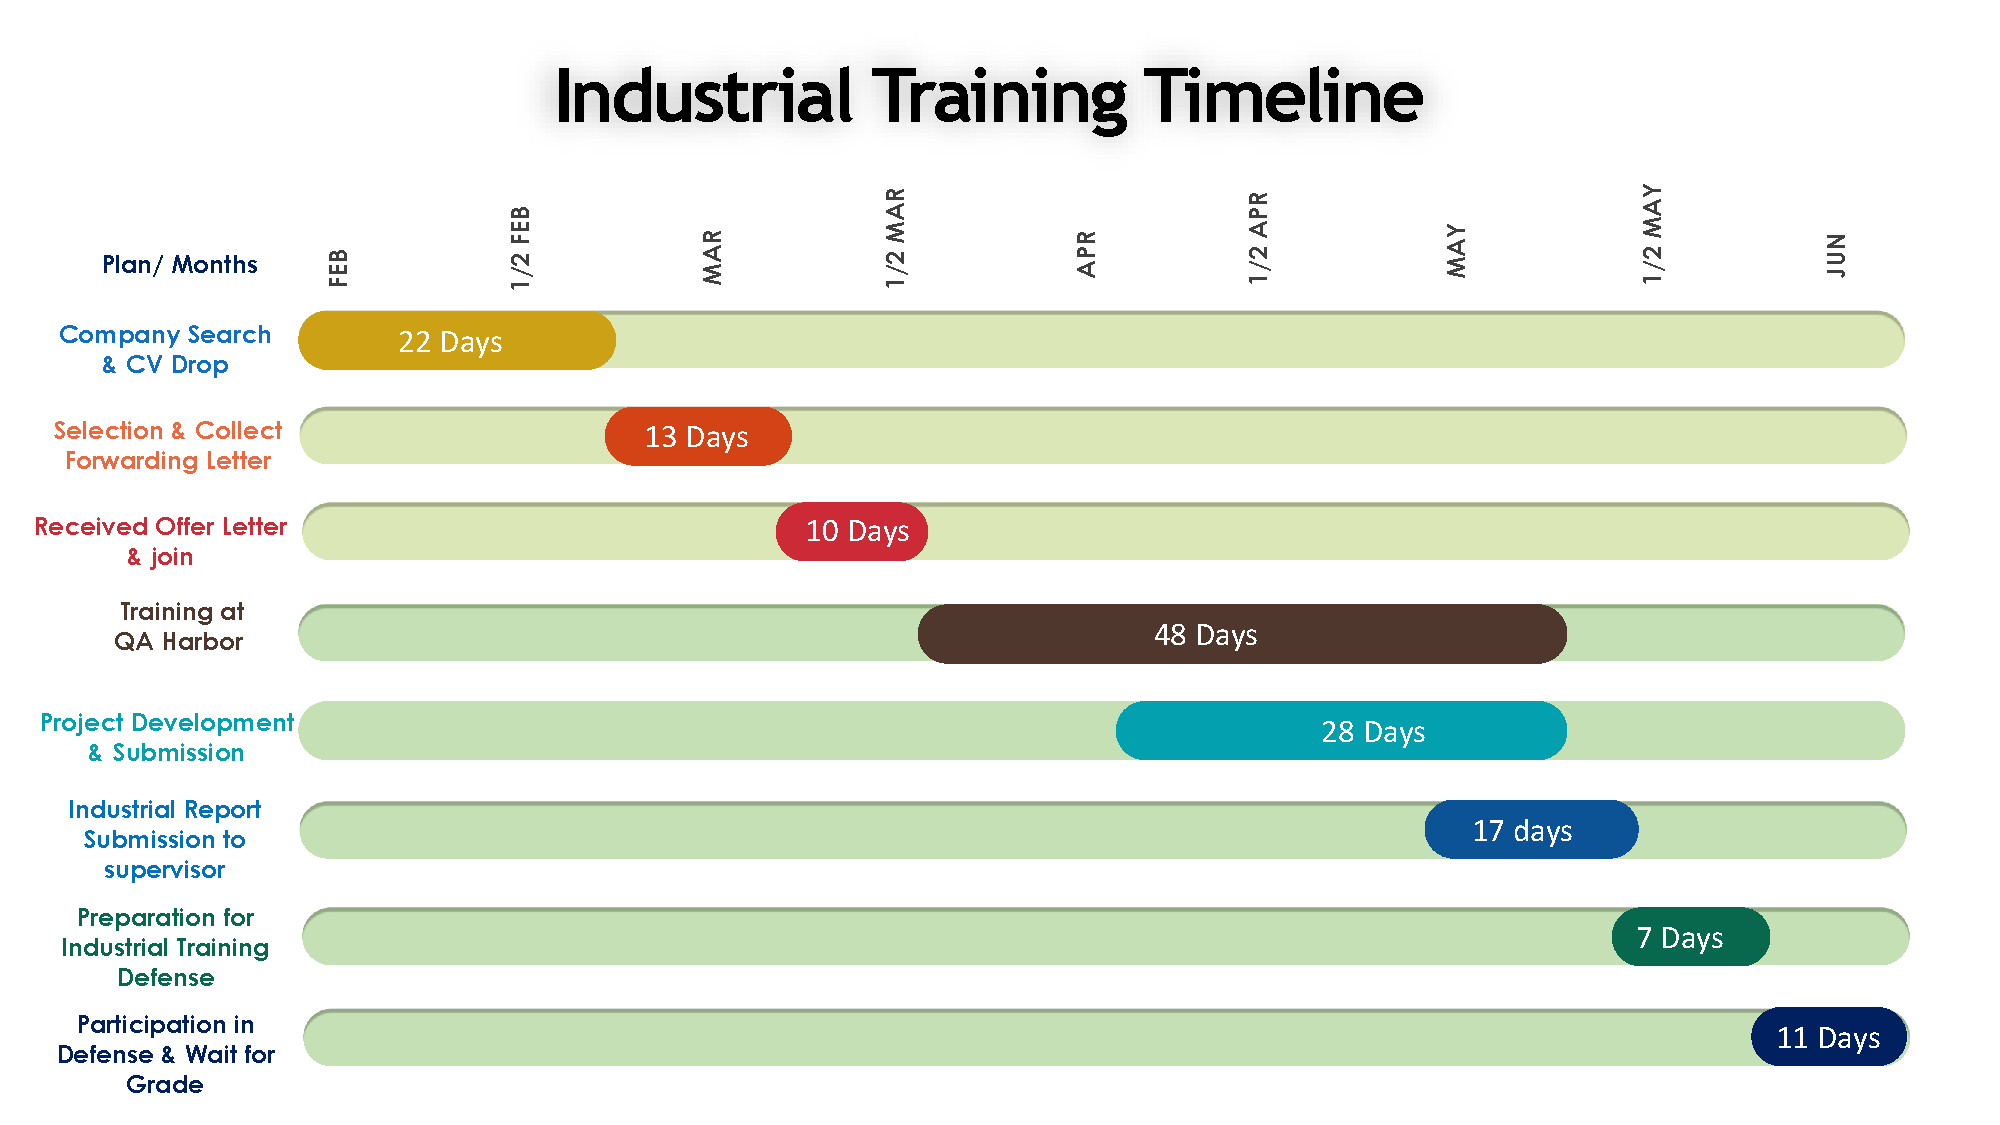
\includegraphics[width=1\linewidth]{figures/Whole Industrial Training Timeline.pdf}
    \caption{Time Management of the Industrial Training Process}
    \label{fig:whole_time}
\end{figure}

\section{Risk Analysis and Resolve Process}

\par During the internship, potential risks such as time constraints, technical difficulties, and communication barriers were identified and managed proactively following a standard risk management process comprising identification, assessment, mitigation, and monitoring (see Figure \ref{fig:risk}).

% 
\textcolor{red}{(You have to refer and describe every Figure you mentioned in your report like above)}

\begin{figure}[H]
    \centering
    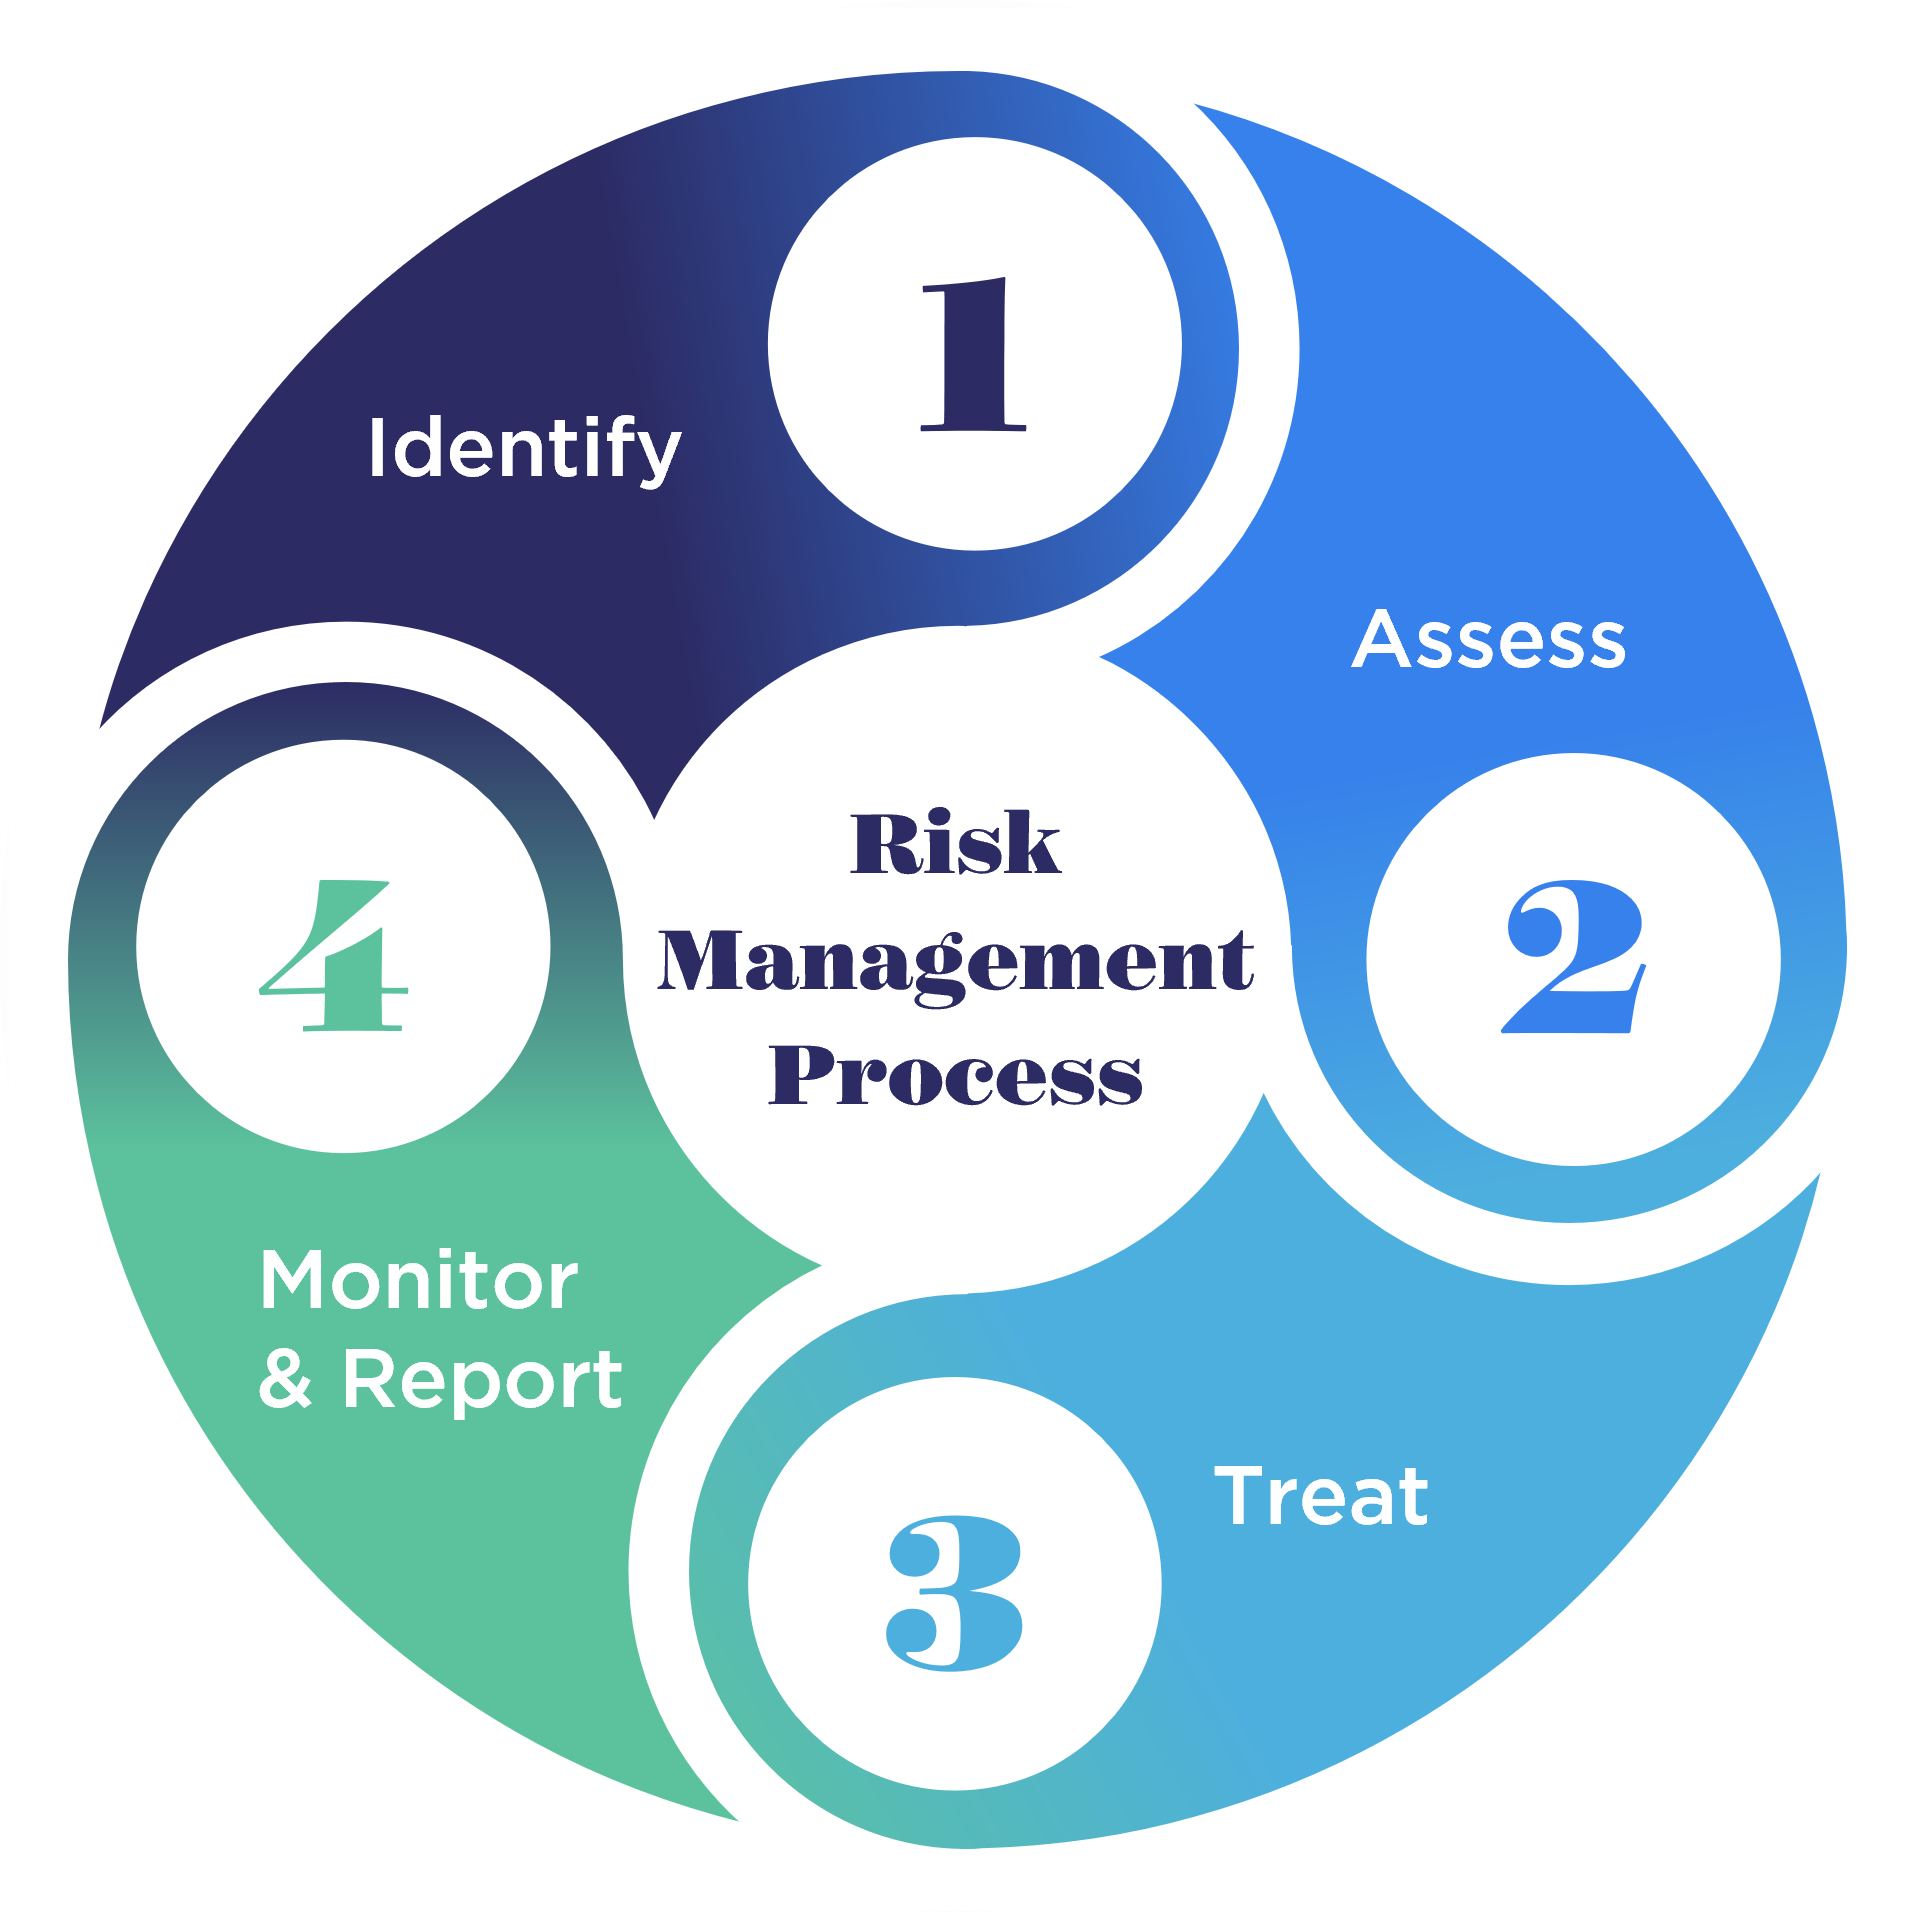
\includegraphics[width=0.3\linewidth]{figures/Four-Steps-of-the-Risk-Management-Process-1 (1).png}
    \caption{Four Steps of the Risk Management Process}
    \label{fig:risk}
\end{figure}

\section{Industrial Training Report Outline}

\begin{itemize}
    \item \textbf{Chapter 2:} Organization Overview – Company structure, services, and mission.
    \item \textbf{Chapter 3:} Training Overview – Key activities, tools, and methodologies applied.
    \item \textbf{Chapter 4:} Skills Acquired – Summary of technical and soft skills developed.
    \item \textbf{Chapter 5:} Conclusion – Reflections, challenges, and recommendations.
\end{itemize}

\section{Conclusion}

\par Industrial training is a vital component in bridging the gap between academic studies and professional work life. It equips students with practical skills, industry exposure, and a better understanding of workplace dynamics. This experience prepares interns for successful careers and enhances their readiness for future challenges in their respective fields.


\chapter{Organization Overview}
\label{chapter-2}

\section{Introduction}
\par [Company Name] is a modern firm committed to providing holistic [industry/sector] solutions. With strong commitments to excellence, precision, and customer success, the organization ensures its products, processes, and systems deliver exceptional quality and reliability. Combining technological expertise with industry knowledge, [Company Name] helps clients improve operational efficiency, mitigate risks, and exceed customer expectations.

\section{Company Profile}
\par \textbf{[Company Name]} is a leading [industry] solutions provider helping businesses of all sizes achieve superior performance. Headquartered at [Location], the company is built on core values including integrity, excellence, innovation, and client-centricity. Founded in [Year], it has grown to [Number] qualified employees, offering innovative solutions across [Region/Country].

\subsection{Certifications}
\begin{table}[H]
\centering
\caption{Company Certifications}
\begin{tabular}{|l|p{5cm}|p{6cm}|}
\hline
\textbf{Certification} & \textbf{Details} & \textbf{Significance} \\
\hline
Example 1 & Description & Business impact \\
\hline
\end{tabular}
\label{tab:certifications}
\end{table}

\subsection{Historical Timeline}
\begin{itemize}
    \item Founding and key milestones
    \item Service expansions
    \item Recent developments
\end{itemize}

\subsection{Work Environment}
\par The company fosters a [describe culture] environment with [list key features]. Employees benefit from [mention perks] while management continuously works to improve [mention areas].

\subsection{Mission and Vision}
\begin{itemize}
    \item \textbf{Mission:} Core commitments and value proposition
    \item \textbf{Vision:} Future aspirations and industry goals
\end{itemize}

\subsection{Core Values}
\begin{itemize}
    \item Quality standards
    \item Customer focus
    \item Innovation
    \item Teamwork
    \item Ethics
\end{itemize}

\section{Organizational Structure}

\textcolor{red}{Organizational structure (i.e. Enterprise or Startup, or etc.) and your interactions with various departments, including collaboration with team leads and cross-functional coordination. This involves regular communication with other departments to understand their responsibilities, align on goals, and support interdepartmental workflows effectively.}

\par The company's structure ensures operational efficiency through clear roles and departmental collaboration. Figure \ref{fig:company-structure} shows the hierarchical breakdown.

\begin{figure}[H]
    \centering
    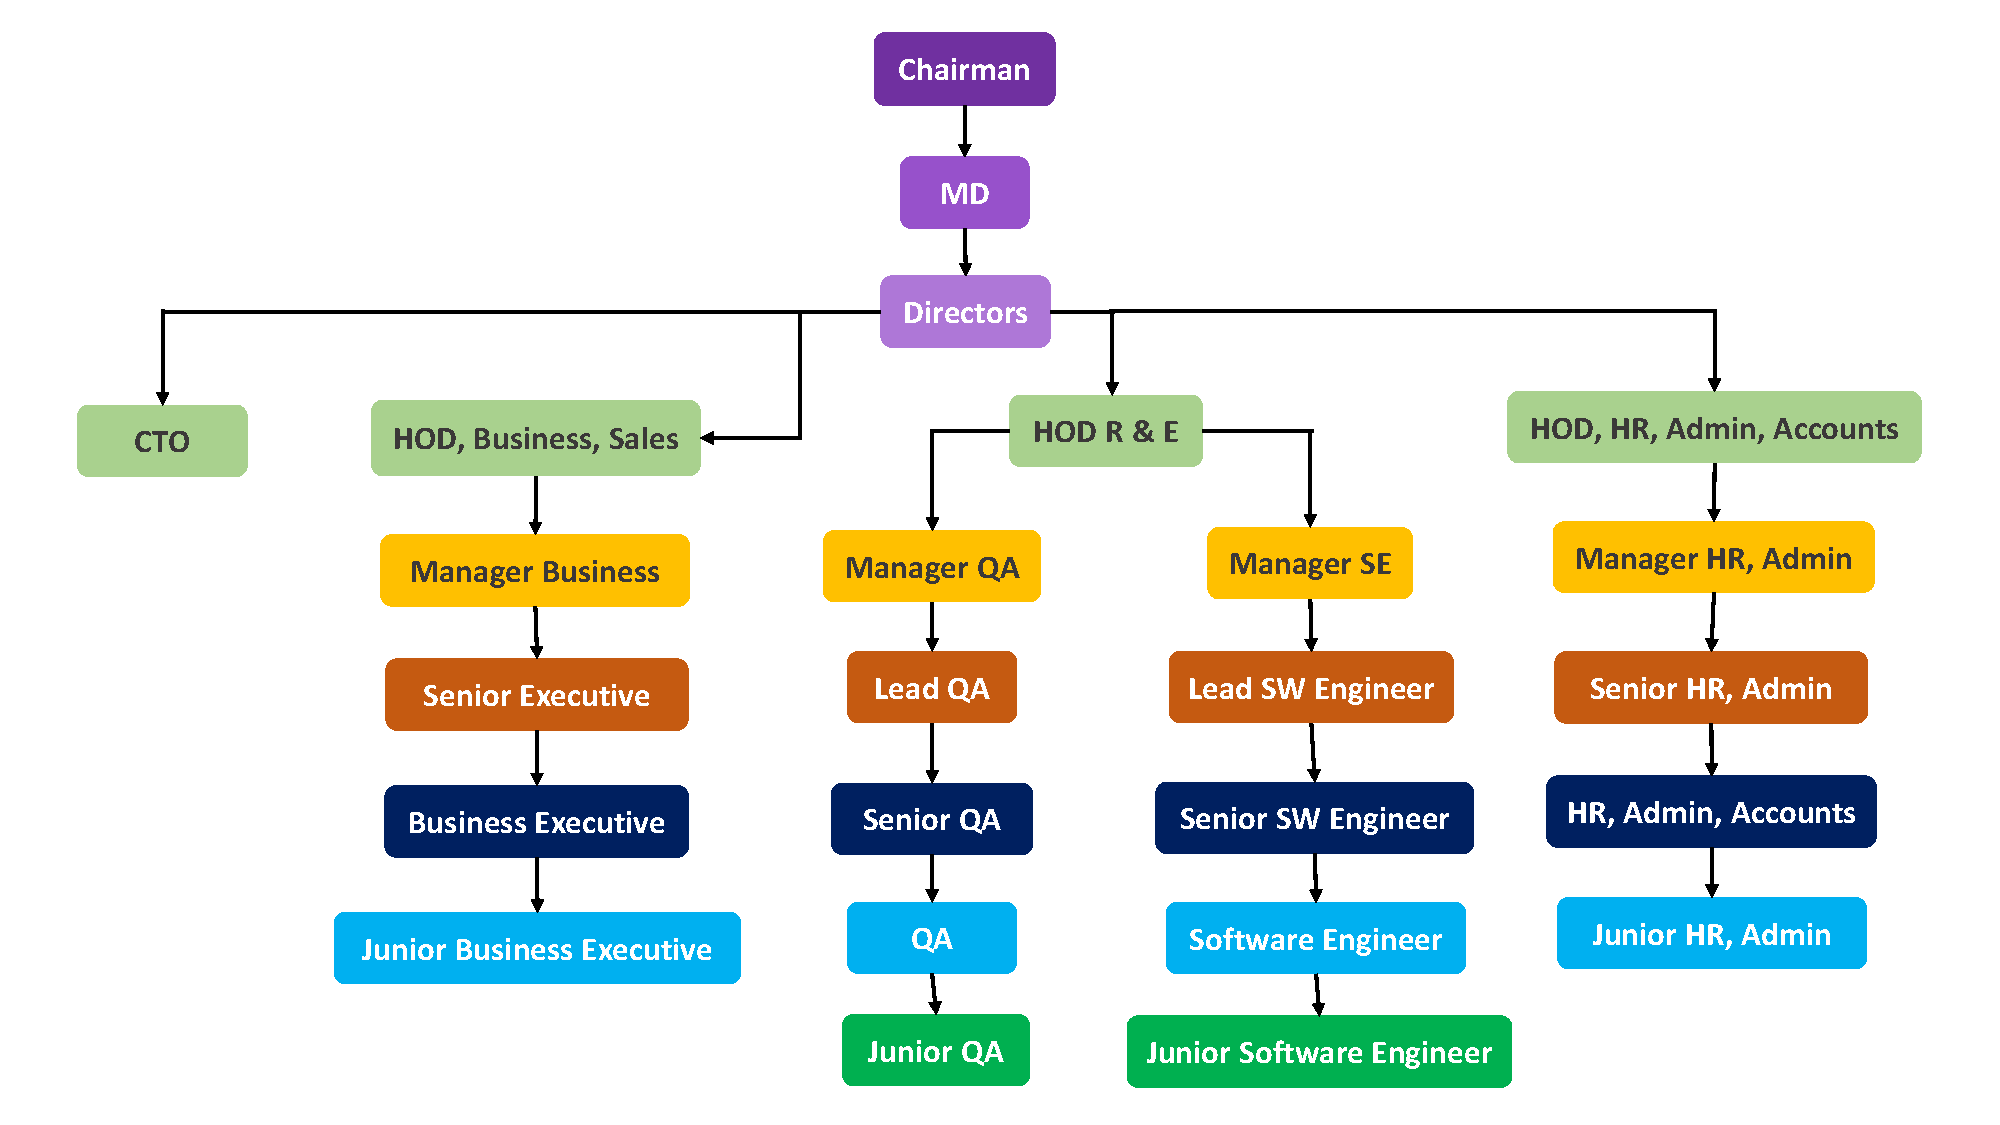
\includegraphics[width=1.0\linewidth]{figures/Company.pdf}
    \caption{Organization Structure}
    \label{fig:company-structure}
\end{figure}

\subsection{Type of Organization}
\par The company operates as a \textit{[Enterprise/Startup/Hybrid]} model, influencing its pace of decision-making, flexibility in processes, and hierarchy depth. This structure defines how projects are prioritized, how resources are allocated, and how quickly initiatives move from concept to execution.

\subsection{Hierarchical Overview}
\begin{itemize}
    \item \textbf{Executive Leadership:} Provides strategic direction.
    \item \textbf{Department Heads:} Lead operational units.
    \item \textbf{Technical Teams:} Implement core solutions.
    \item \textbf{Support Functions:} Handle HR, admin, and finance.
\end{itemize}

\subsection{Roles and Responsibilities of Officials}
\begin{itemize}
    \item \textbf{Chief Executive Officer (CEO):} Sets overall strategic vision, ensures organizational goals align with market opportunities, and represents the company to external stakeholders.
    \item \textbf{Chief Operating Officer (COO):} Oversees day-to-day operations, manages cross-departmental workflows, and ensures operational efficiency.
    \item \textbf{Chief Technology Officer (CTO):} Leads technology strategy, oversees development teams, and ensures that technical solutions meet business requirements.
    % Add other roles as needed
    \newline
    ...
\end{itemize}

\subsection{Interactions with Various Departments}
\par Daily operations involve engagement with multiple departments. Each department has clearly defined responsibilities, and regular communication ensures mutual awareness of progress, challenges, and dependencies.

\subsection{Collaboration with Team Leads}
\par Team leads serve as the primary coordination points within their functional areas. Regular sync meetings, sprint reviews, and project status updates help align technical deliverables with business objectives.

\subsection{Cross-Functional Coordination}
\par Many initiatives span across technical, product, and support teams. Structured workflows—such as shared project boards, standardized reporting formats, and agreed escalation paths—enable smooth collaboration between functions.

\subsection{Interdepartmental Communication}
\par Consistent communication channels, including weekly cross-departmental meetings, collaborative documentation platforms, and direct messaging tools, help maintain alignment and resolve issues before they impact delivery timelines.



\section{Products/Services}
\textcolor{red}{Provide detailed information about a product or service, including its methodology, any relevant diagrams such as ER (Entity-Relationship) diagrams or UI (User Interface) designs. You may choose a product/service that is well-known, widely used, or one you are familiar with.}
\begin{itemize}
    \item \textbf{Details} [General description]
    \item \textbf{Specialized Services:} [General description]
    \item \textbf{Training Programs:} [General description]
\end{itemize}



\section{Clients}
\begin{itemize}
    \item Representative clients across industries
    \item Confidentiality note regarding unnamed clients
\end{itemize}


\section{Direct Involvement of Resources During Training }
\begin{itemize}
    \item \textbf{Human Resources:}
    \begin{itemize}
        \item Mentors and supervisors
        \item Training personnel
        \item Leadership access
    \end{itemize}
    \item \textbf{Technical Resources:}
    \begin{itemize}
        \item Work equipment
        \item Software tools
        \item Testing platforms
    \end{itemize}
\end{itemize}


\section{Constructive Feedback About the Training Program}
\begin{itemize}
    \item Provide balanced feedback:
    \begin{itemize}
        \item Positive aspects of the experience
        \item Areas for improvement
        \item Suggestions for future interns
    \end{itemize}
    \item Maintain professional tone
    \item Focus on learning outcomes
\end{itemize}

\section{Conclusion}
\par [Company Name] is a [type] organization specializing in [key services]. With its [describe structure] and focus on [key values], the company maintains industry standards while contributing to sector growth. The organization's commitment to [highlight principle] makes it an ideal environment for professional development.
\chapter{Specific Details on Training Activities and Report}
\label{chapter-3}

% Include:
% - Actual weekly activities performed
% - Specific tools used (replace examples)
% - Personal learning experiences
% - Project details with quantifiable outcomes

\section{Introduction}
\begin{itemize}
    \item Brief overview of the internship duration and host organization
    \item Key learning objectives and focus areas
    \item Technologies/tools used during training
    \item Summary of professional growth
\end{itemize}

\section{Weekly Duties and Activities}

\subsection{First Week: Overall Activity / Topic Name (e.g. Foundation)}
\begin{itemize}
    \item \textbf{Orientation:} Company introduction and team onboarding
    \item \textbf{Key Concepts Learned:}
    \begin{itemize}
        \item Software testing fundamentals
        \item SDLC (Stages as mentioned Fig.~\ref{fig:sdlc}), and STLC methodologies
        \item Testing types (manual/automation)
    \end{itemize}
\end{itemize}

\textcolor{red}{(You have to refer and describe every Figure you mentioned in your report like above)}

\begin{figure}[H]
    \centering
    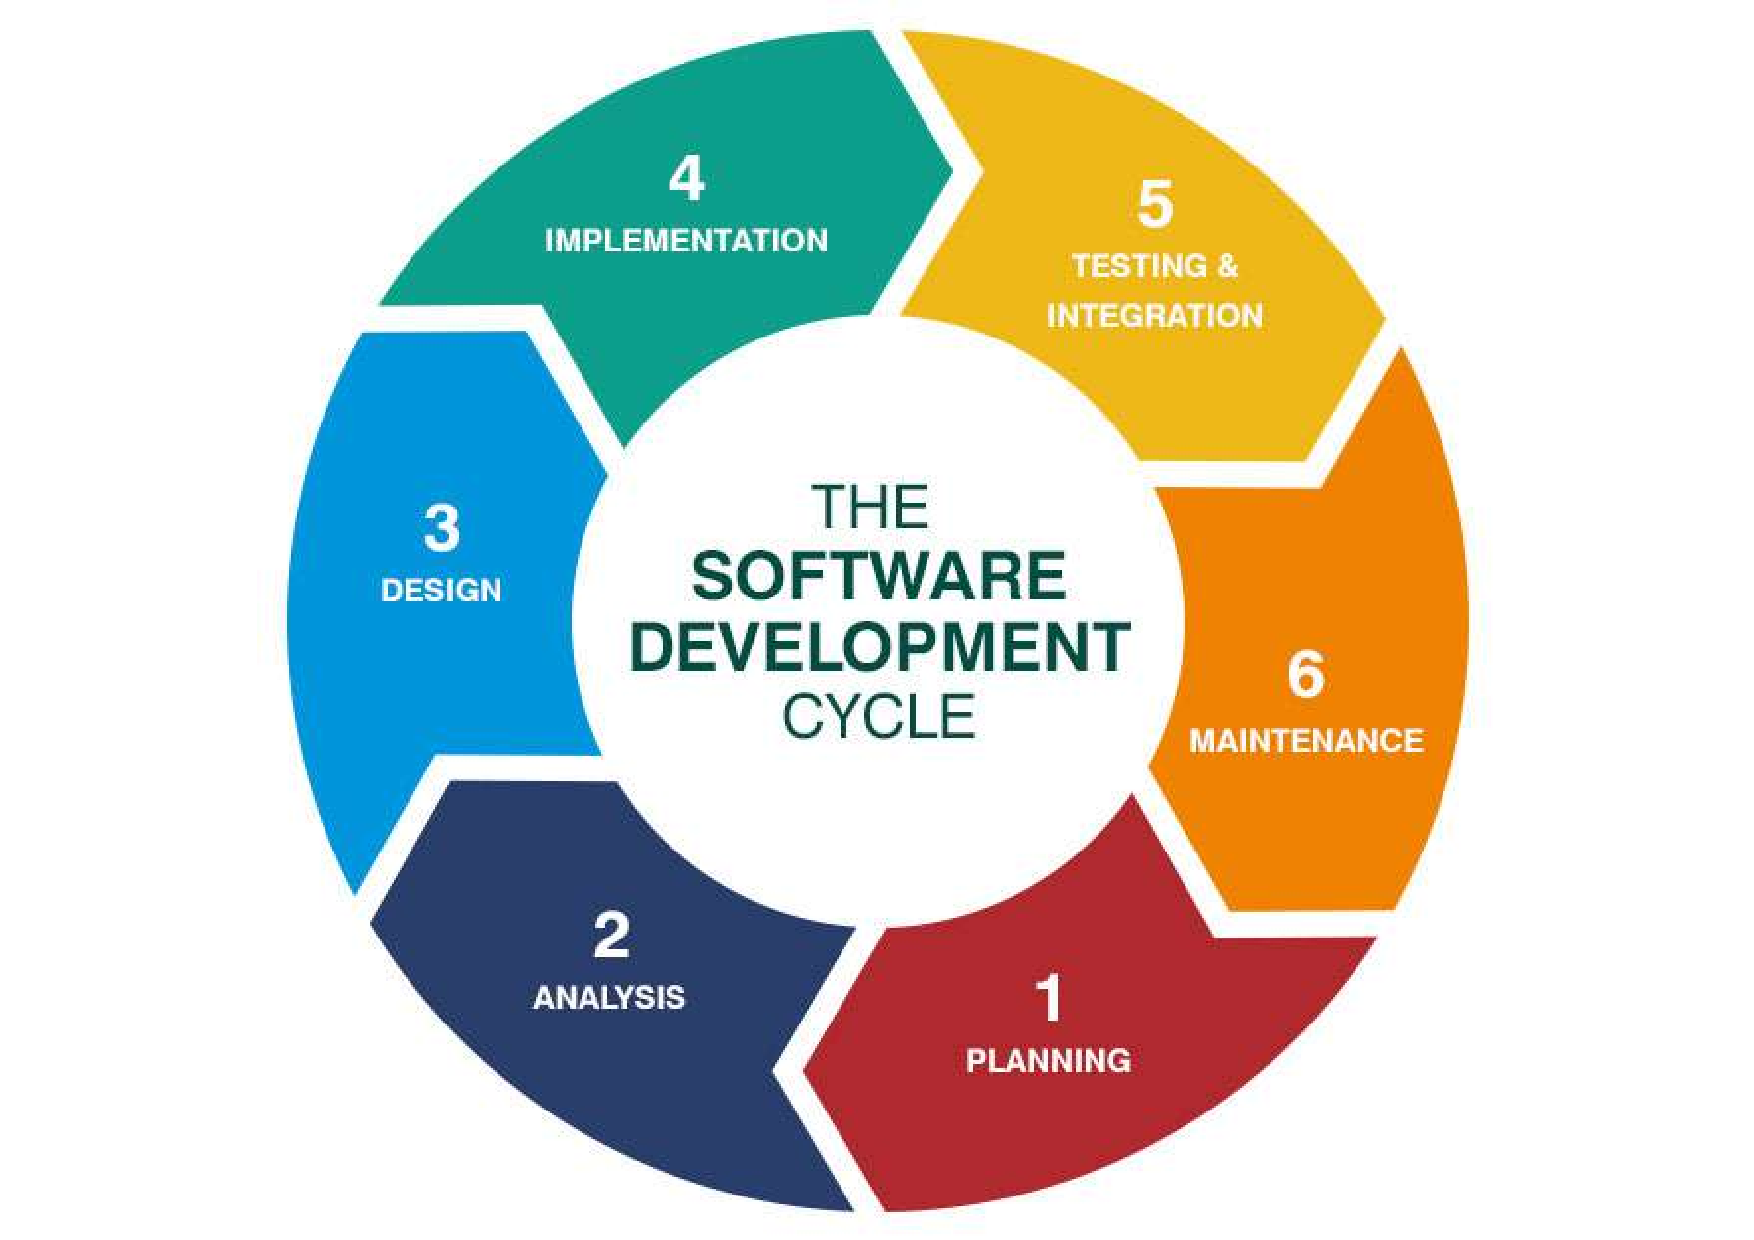
\includegraphics[width=0.6\linewidth]{figures/SDLC-stages.pdf}
    \caption{SDLC Stages (Replace with actual diagram)}
    \label{fig:sdlc}
\end{figure}

\subsection{Second Week:  Overall Activity / Topic Name (e.g. Practical Applications)}
\begin{itemize}
    \item \textbf{Hands-on Training:}
    \begin{itemize}
        \item Test case design and execution (See Table~\ref{tab:test-case-template}) \textcolor{red}{(You have to refer and describe every Table you mentioned in your report like above)}
        \item Bug reporting workflows
        \item Agile methodologies
    \end{itemize}
    \item \textbf{Tools Introduced:} Playwright, Postman
\end{itemize}

\begin{table}[H]
\centering
\caption{Sample Table}
\begin{tabular}{|l|p{8cm}|}
\hline
\textbf{Component} & \textbf{Description} \\ \hline
Test Case ID & Unique identifier \\ \hline
Test Scenario & Brief description \\ \hline
Test Steps & Detailed actions \\ \hline
Expected Result & Anticipated outcome \\ \hline
\end{tabular}
\label{tab:test-case-template}
\end{table}

\subsection{Third Week: Overall Activity / Topic Name (e.g. Automation)}
\begin{itemize}
    \item \textbf{Page Object Model:}
    \begin{itemize}
        \item Architecture design
        \item Implementation strategy
    \end{itemize}
    \item \textbf{Project Structure:}
    \begin{lstlisting}[style=tree]
project/
|-- pages/
|-- tests/
|-- utilities/
|-- .../
|-- .../
    \end{lstlisting}
\end{itemize}

\subsection{Fourth Week: Overall Activity / Topic Name (e.g. Advanced Concepts)}
\begin{itemize}
    \item \textbf{API Testing:} REST principles and practical implementation
    \item \textbf{Performance Testing:} JMeter fundamentals
    \item \textbf{Version Control:} Git/GitHub workflows
\end{itemize}

\section{Key Projects}
\textcolor{red}{You must include workflow diagrams, ER diagrams, or sequence/class diagrams, or alternatively, add screenshots of the projects you worked on during your internship. If any screenshots contain sensitive information, ensure you have proper authorization before including them. Additionally, clearly mention your role and contributions to the project, any models used, the outcomes achieved, and the business perspective or impact of the project.}
\subsection{Project 1: Web Application Testing} 
    \begin{itemize}
        \item Scope and objectives
        \item ER and related diagrams
        \item Tools used
        \item Outcomes
    \end{itemize}
    
\subsection{Project 2: API Test Automation} 
    \begin{itemize}
        \item Test coverage
        \item ER and related diagrams
        \item Challenges faced
        \item Solutions implemented
    \end{itemize}

\subsection{Project 3: ...}

\textcolor{red}{You must include Entity-Relationship (ER) diagrams and related diagrams similar to IDP2. If company policies restrict the use of original diagrams, you should use replica diagrams instead.}

% \section{Automation Testing Example}
% Below is a complete Python test automation script using Playwright that students can include in their report:

% \newpage

% \begin{lstlisting}[language=Python, caption={Demo Python Script}, label=code:demo]

% import pandas as pd

% def drop_row(csv_filename):
%     """Read a CSV file and dropped the first row"""
%     df = pd.read_csv(csv_filename)
%     return df.drop(0)

% df = drop_row("demo.csv")
% \end{lstlisting}

% Key Features Demonstrated:
% \begin{itemize}
%     \item Complete working test script
%     \item Browser automation with Playwright
%     \item Common test actions (navigation, assertions)
%     \item Proper error handling
%     \item Page object pattern basics
% \end{itemize}

% \textcolor{red}{This below section is optional}

\section{Other Responsibilities}

\textcolor{red}{(e.g. Team Management, Proposal Writing)}

\section{Key Performance Indicator}
\textcolor{red}{If you achieved any KPIs during your internship, be sure to include them with sufficient and relevant evidence.}

\section{Internship Summary}

\textcolor{red}{Mention bit details about your summary and learning, not necessarily exact to the below given format}

\par The industrial internship was a mandatory component of the undergraduate B.Sc. in Computer Science and Engineering program. It aimed to provide practical exposure and a real-world working environment to enhance academic learning with hands-on experience. The training focused on the application of theoretical knowledge to software development, debugging, collaboration, and use of modern tools in a professional setting.

\par The internship was conducted in a hybrid mode, combining remote project-based tasks with periodic in-person meetings for review and feedback. A variety of learning methodologies were adopted, including self-paced assignments, team collaboration, live mentoring sessions, and peer code reviews. The experience helped in developing technical competency, improving communication skills, and strengthening ethical awareness.

\textcolor{red}{Clearly mention the exact table rows along with your specific accomplishments and details.}

\par The key summary of the internship is presented in Table~\ref{tab:internship-summary}.

\begin{table}[H]
\centering
\caption{Internship Summary}
\label{tab:internship-summary}
\renewcommand{\arraystretch}{1.4}
\begin{tabularx}{\textwidth}{|>{\centering\arraybackslash}p{5cm}|>{\arraybackslash}X|}
\hline
\textbf{Parameter} & \textbf{Details} \\
\hline
\textbf{Organization Name} & [Insert Company/Organization Name] \\
\hline
\textbf{Internship Period} & [Insert Start Date] to [Insert End Date] \\
\hline
\textbf{Total Duration} & [e.g., 8 weeks (56 days)] \\
\hline
\textbf{Total Working Hours} & [e.g., 320 hours (approx.)] \\
\hline
\textbf{Mode of Internship} & Hybrid (Remote + Onsite) \\
\hline
\textbf{Nature of Work} & Software Development, Testing, Debugging, Documentation \\
\hline
\textbf{Tools and Technologies Used} & Git, Postman, JMeter, Firebase, Docker, SQL, JavaScript \\
\hline
\textbf{Learning Methodology} & Self-paced tasks, Live mentoring, Code reviews, Weekly stand-up meetings \\
\hline
\textbf{Reporting Mechanism} & Weekly progress reports and final project presentation \\
\hline
\textbf{Mentor/ Supervisor} & [Insert Mentor’s Name and Designation] \\
\hline
\end{tabularx}
\end{table}


\textcolor{red}{Mention a concluding summary of your learning in 3-4 lines, not necessarily exact to the below given format}

\par Overall, the internship provided a comprehensive platform to integrate academic concepts with practical industrial processes. It contributed significantly to the development of professional behavior, time management, technical proficiency, and alignment with Sustainable Development Goals (SDGs).

% \section{Conclusion}
% \begin{itemize}
%     \item Summary of key experiences
%     \item How training aligned with academic knowledge
%     \item Future application of learned skills
% \end{itemize}
\chapter{Acquired Skills During Industrial Training}
\label{chapter-4}

\section{Introduction}
\begin{itemize}
    \item Briefly describe your industrial training program and host organization
    \item State the duration and key focus areas of your training
    \item Highlight how this experience bridged academic learning with practical application
    \item Example: "The industrial training at [Company Name] provided hands-on experience in [...]"
\end{itemize}

\section{Learning New Technologies and Applying Them to Solve Engineering Problems}
\begin{itemize}
    \item List all major technologies/tools learned during training
    \item For each technology:
    \begin{itemize}
        \item Describe your proficiency level (basic/intermediate/advanced)
        \item Provide specific examples of problems solved
        \item Mention any certifications or special training received
    \end{itemize}
    \item Include quantitative achievements where possible (e.g., "Automated 25+ test cases")
\end{itemize}

\section{Theoretical Knowledge Gained}
\begin{itemize}
    \item Outline key theoretical concepts learned
    \item Organize by categories:
    \begin{itemize}
        \item Software testing principles
        \item Development methodologies
        \item Testing types and techniques
    \end{itemize}
    \item Connect each concept to practical applications
\end{itemize}

\section{Practical Knowledge Acquired}

\textcolor{red}{You must describe your experience and the knowledge you gained from the industrial training program. Explain how you could use this experience to start a startup similar to the company where you worked. Additionally, discuss the resources required (hardware, human resources), budgeting considerations, and the type of project you could undertake to leverage this internship experience for launching your own company.}

\begin{itemize}
    \item Detail hands-on experiences:
    \begin{itemize}
        \item Test case design and execution
        \item Defect tracking processes
        \item Tools used for various testing types
        \item Team collaboration methods
    \end{itemize}
    \item Include specific examples from projects
\end{itemize}

\section{Communication Skills Developed}
\begin{itemize}
    \item Describe how communication skills improved:
    \begin{itemize}
        \item Technical reporting
        \item Team meetings
        \item Client/stakeholder interactions
    \end{itemize}
    \item Provide examples of effective communication
    \item Mention any challenges overcome
\end{itemize}

\section{Collaboration Skills Enhanced}
\begin{itemize}
    \item Explain teamwork experiences:
    \begin{itemize}
        \item Cross-functional projects
        \item Pair programming/testing
        \item Knowledge sharing sessions
    \end{itemize}
    \item Highlight leadership opportunities
    \item Discuss conflict resolution examples
\end{itemize}

\section{Ethical Responsibilities and Professional Conduct}
\begin{itemize}
    \item Discuss ethical considerations encountered
    \item Reference the IEEE Code of Ethics table (Table \ref{tab:ieee-ethics-mapping})
    \item Provide specific examples of ethical decision-making
    \item Describe how professional standards were maintained
\end{itemize}

\begin{table}[H]
\centering
\caption{IEEE Code of Ethics Applied During Industrial Training}
\begin{adjustbox}{width=0.9\textwidth}
\begin{tabular}{|l|p{10cm}|}
\hline
\textbf{IEEE Code} & \textbf{Implementation in Training} \\ \hline
\textbf{Public Safety \& Welfare} & Describe how you ensured user safety and data privacy \\ \hline
\textbf{Professional Integrity} & Examples of honest reporting and conflict avoidance \\ \hline
\textbf{Fairness \& Inclusion} & How you promoted equitable testing practices \\ \hline
\textbf{Technical Competence} & Steps taken to maintain and improve skills \\ \hline
\end{tabular}
\end{adjustbox}
\label{tab:ieee-ethics-mapping}
\end{table}

\section{Conclusion}
\begin{itemize}
    \item Summarize key skills gained
    \item Reflect on personal/professional growth
    \item Connect to future career goals
    \item Example: "This training has prepared me for [...]"
\end{itemize}
\chapter{Conclusion}
\label{chapter-5}

\section{Summary}

\par The industrial training program at Active Green Energy Ltd. was an invaluable opportunity to bridge the gap between academic education and practical industry experience. Over the course of the internship, I gained comprehensive exposure to a real business analysis and digital-solutions role, working on two parallel industrial digital product concepts: an Industrial Energy \& Machinery Monitoring System and an IIoT-Based Production Monitoring System. The training enabled me to apply theoretical knowledge in requirements engineering and system design, learn industry-standard tools such as Figma and Jira, and improve my problem-solving and stakeholder-communication skills.

\par This experience enhanced both my technical competencies and professional development. I gained a deeper understanding of how requirements move from a client conversation to a documented specification, then to a design, and finally to a working prototype, as well as how to collaborate with designers, developers, and testers along the way. Overall, the training served as a significant milestone in preparing me for future career opportunities in business analysis and digital solution design.


\section{Challenges During Industrial Training}
\par During the internship, I encountered several challenges that contributed to my learning and growth. Adapting to the company's documentation standards, translating ambiguous client requirements into structured specifications, and coordinating between business and technical stakeholders were all part of the experience.

\par Some specific challenges faced included:
\begin{enumerate}
    \item \textbf{Understanding Incomplete Requirements:} Early client discussions did not always translate directly into clear, testable requirements, requiring follow-up questions and iterative refinement of the SRS/PRD documents.
    \item \textbf{Learning New Tools Quickly:} Becoming proficient with Figma, Jira, and AI-assisted development tools such as Claude Code within a short time frame, while still producing usable output for live projects.
    \item \textbf{Managing a Real Project Delay:} On the IIoT-Based Production Monitoring System project, a delayed factory visit by the IoT engineering team pushed back device setup and the overall timeline, requiring me to help communicate the delay to the client professionally and manage revised expectations.
    \item \textbf{Balancing Two Concurrent Projects:} Dividing attention and documentation effort between two active projects while maintaining consistent quality in both.
    \item \textbf{Validating AI-Assisted Output:} Learning to treat AI-generated prototypes as a starting point requiring careful review against requirements, rather than a finished deliverable.
\end{enumerate}

\section{Scope of the Study}
\par The internship focused on applying and enhancing both academic knowledge and professional skills within the specific domain of business analysis and digital solution design. The following key areas were explored:

\begin{itemize}
    \item \textbf{Understanding Industry Workflows:} Exposure to how requirements, design, and prototyping work in a real industrial technology company.
    \item \textbf{Technical Skill Development:} Practical experience with requirements documentation, system diagramming, UI/UX design, and AI-assisted prototyping tools.
    \item \textbf{Team Collaboration and Communication:} Working with a supervisor, designers, developers, and testers in a coordinated, goal-oriented manner.
    \item \textbf{Professionalism and Ethics:} Learning to communicate difficult news (such as project delays) transparently and professionally.
    \item \textbf{Problem-Solving and Adaptability:} Facing ambiguous requirements and schedule risks, and adapting plans accordingly.
\end{itemize}

\section{Problems and Executions}
\par Throughout the internship, I engaged in tasks that allowed me to apply my academic training in a practical setting -- from requirements analysis coursework to real client requirement-gathering, and from diagramming exercises to production-quality DFD, Use Case, and ER diagrams for live projects.

\par With guidance from my supervisor, I learned how to:
\begin{itemize}
    \item Analyze client requirements and translate them into structured SRS/PRD documentation.
    \item Design system workflows and UI/UX concepts that reflected those requirements accurately.
    \item Use AI-assisted tools to accelerate prototyping while independently validating the results.
    \item Communicate project risks and delays to clients honestly and constructively.
\end{itemize}

\par These experiences helped strengthen my technical foundations in requirements engineering and system design, and taught me how to remain adaptable and solution-oriented when real projects did not go exactly as planned.

\section{Overall Achievement}
\par In conclusion, the internship provided a well-rounded learning experience, helping me grow both as a student and as a future business analyst. I improved my requirements-engineering and UI/UX design skills, gained hands-on experience with AI-assisted development workflows, and learned how to communicate effectively with both technical and non-technical stakeholders. I am particularly proud of successfully carrying both assigned projects from initial requirement gathering through to working prototypes, and of managing the client communication around the IIoT project's delay without it derailing the relationship.

\par If I were to approach the internship again, I would try to establish a lightweight personal log of client feedback and decisions from week one, rather than relying on memory and scattered notes -- a habit I plan to carry into future roles. Overall, the training reinforced my academic learning while introducing me to the practical realities of business analysis, and it has laid a solid foundation for my future career in digital solution design.

\clearpage
\chapter*{Annexure: Graduate Map Program Outcome (PO) with Skill Achievement from Industrial Training}
\addcontentsline{toc}{chapter}{Annexure: PO-Skill Mapping}

\par Program Outcomes (POs) \cite{16} serve as critical benchmarks to measure the knowledge, skills, and competencies acquired during my B.Sc. in CSE journey, ensuring alignment between academic curricula and industry demands. While universities focus on theoretical knowledge, Program Outcomes (POs) ensure graduates possess the technical, problem-solving, and ethical skills needed in the industry. During my industrial training, I had the opportunity to apply Computer Science \& Engineering knowledge in real-world scenarios, such as testing, debugging, collaboration, and adhering to ethical standards. This experience bridged the gap between theory and practice, enhanced my technical proficiency, and strengthened my soft skills.

\par Mapping POs is essential to evaluate how well academic learning translates to industry practice. Three core reasons for mapping these outcomes include:
\begin{itemize}
    \item To assess curriculum relevance to industrial expectations,
    \item To evaluate readiness in applying theory to practical tools and technologies, and
    \item To enable self-assessment of professional and ethical growth.
\end{itemize}

\par The following Table~\ref{tab:po-fulfillment} maps the 12 Program Outcomes (POs) with the knowledge and skills acquired through both academic education and industrial training. Fulfillment level indicates how effectively each PO was addressed during the internship.

\begin{longtable}[H]{|p{2.5cm}|p{3.5cm}|p{2cm}|p{4cm}|p{4cm}|}
\caption{Program Outcome (PO) Fulfillment in Industrial Training} \label{tab:po-fulfillment} \\
\hline
\textbf{PO} & \textbf{Description} & \textbf{Fulfillment Level} & \textbf{Training Knowledge Applied} & \textbf{Evidence} \\
\hline
\endfirsthead

\multicolumn{5}{c}%
{{\bfseries \tablename\ \thetable{} -- continued from previous page}} \\
\hline
\textbf{PO} & \textbf{Description} & \textbf{Fulfillment Level} & \textbf{Training Knowledge Applied} & \textbf{Evidence} \\
\hline
\endhead

\hline \multicolumn{5}{r}{{Continued on next page}} \\
\endfoot

\hline
\endlastfoot

\textbf{PO2: Problem Analysis} & Identify, formulate, and analyze complex computing problems. & Fully Fulfilled & Diagnosed root causes of bugs and performance issues in software systems. & Identified a bottleneck in backend queries that improved application speed by 30\%. \\
\hline

\textbf{PO5: Modern Tools} & Apply theoretical understanding of modern tools. & \textit{[Insert Fulfillment Level]} & \textit{[Mention tools used: Git, Postman, JMeter, etc.]} & \textit{[Describe a task or tool automation achieved]} \\
\hline

\textbf{PO6: Engineer \& Society} & Understand societal implications of computing solutions. & \textit{[Insert Fulfillment Level]} & \textit{[Mention any user-data, privacy, or accessibility work]} & \textit{[Evidence of ensuring societal responsibility]} \\
\hline

\textbf{PO7: Environment} & Evaluate environmental impact of computational systems. & Not Fulfilled & N/A & Environmental aspects were not addressed in the assigned project. \\
\hline

\textbf{PO8: Ethics} & Apply ethical theories in decision-making. & Fully Fulfilled & Ensured accuracy in documentation, refused unethical shortcuts. & Reported a misconfiguration instead of bypassing it for faster testing. \\
\hline

\textbf{PO10: Communication} & Communicate technical concepts clearly. & \textit{[Insert Fulfillment Level]} & \textit{[Describe presentation, reporting, or documentation]} & \textit{[Mention audience and feedback or result]} \\
\hline

\textbf{PO12: Lifelong Learning} & Recognize the need for continuous learning. & Fully Fulfilled & Explored a new technology (e.g., Docker, Firebase, or AI testing). & Completed an online course and implemented learned skills in a demo module. \\
\end{longtable}

\begin{longtable}[H]{|p{1.5cm}|p{4cm}|p{4cm}|p{4cm}|}
\caption{Complex Engineering Problems (WP) -- Application to Project}
\label{tab:cep} \\
\hline
\textbf{No.} & \textbf{Attribute} & \textbf{Description} & \textbf{How it applies to your problem} \\
\hline
\endfirsthead
\multicolumn{4}{c}{{\bfseries \tablename\ \thetable{} -- continued from previous page}} \\
\hline
\textbf{No.} & \textbf{Attribute} & \textbf{Description} & \textbf{How it applies to your problem} \\
\hline
\endhead
\hline \multicolumn{4}{r}{{Continued on next page}} \\
\endfoot
\hline
\endlastfoot

\multicolumn{4}{|p{13.5cm}|}{%
  \textbf{Complex problems} have characteristic WP1 and some or all of WP2 to WP7.} \\
\hline

%% --- WP1 (mandatory) ---
\textbf{WP1} &
Depth of Knowledge Required &
Cannot be resolved without in-depth engineering knowledge at WK3, WK4, WK5, WK6 or WK8 level, requiring a first-principles analytical approach. &
\toFill{describe what deep knowledge was needed to solve your problem} \\
\hline

%% --- WP2 ---
\textbf{WP2} &
Range of conflicting requirements &
Involve wide-ranging or conflicting technical, engineering and other issues. &
\toFill{describe any conflicting technical or stakeholder requirements faced} \\
\hline

%% --- WP3 ---
\textbf{WP3} &
Depth of analysis required &
Have no obvious solution and require abstract thinking and originality to formulate suitable models. &
\toFill{explain what analysis or modelling approach was needed} \\
\hline

%% --- WP4 ---
\textbf{WP4} &
Familiarity of issues &
Involve infrequently encountered issues. &
\toFill{describe any unusual or unfamiliar issues encountered} \\
\hline

%% --- WP5 ---
\textbf{WP5} &
Extent of applicable codes &
Are outside problems encompassed by standards and codes of practice for professional engineering. &
\toFill{note if the problem went beyond standard codes or guidelines} \\
\hline

%% --- WP6 ---
\textbf{WP6} &
Extent of stakeholder involvement and level of conflicting requirements &
Involve diverse groups of stakeholders with widely varying needs. &
\toFill{list the stakeholders involved and their differing needs} \\
\hline

%% --- WP7 ---
\textbf{WP7} &
Interdependence &
Are high level problems including many component parts or sub-problems. &
\toFill{describe the sub-problems or components that made up the overall problem} \\
\hline

\end{longtable}

\newpage

\begin{longtable}[H]{|p{1.5cm}|p{4cm}|p{4cm}|p{4cm}|}
\caption{Complex Engineering Activities (EA) -- Application to Project}
\label{tab:cea} \\
\hline
\textbf{No.} & \textbf{Attribute} & \textbf{Description} & \textbf{How it applies to your activity} \\
\hline
\endfirsthead
\multicolumn{4}{c}{{\bfseries \tablename\ \thetable{} -- continued from previous page}} \\
\hline
\textbf{No.} & \textbf{Attribute} & \textbf{Description} & \textbf{How it applies to your activity} \\
\hline
\endhead
\hline \multicolumn{4}{r}{{Continued on next page}} \\
\endfoot
\hline
\endlastfoot

\multicolumn{4}{|p{13.5cm}|}{%
  \textbf{Complex activities} mean (engineering) activities or projects that have some or all of the following characteristics.} \\
\hline

%% --- EA1 ---
\textbf{EA1} &
Range of resources &
Involve the use of diverse resources including people, money, equipment, materials, information and technologies. &
\toFill{list the resources used, e.g.\ team members, tools, budget, datasets} \\
\hline

%% --- EA2 ---
\textbf{EA2} &
Level of interactions &
Require resolution of significant problems arising from interactions between wide-ranging or conflicting technical, engineering or other issues. &
\toFill{describe interactions or conflicts between technical components or teams} \\
\hline

%% --- EA3 ---
\textbf{EA3} &
Innovation &
Involve creative use of engineering principles and research-based knowledge in novel ways. &
\toFill{explain any novel or creative approach taken during the activity} \\
\hline

%% --- EA4 ---
\textbf{EA4} &
Consequences to society and the environment &
Have significant consequences in a range of contexts, characterised by difficulty of prediction and mitigation. &
\toFill{describe potential societal or environmental impact of the activity} \\
\hline

%% --- EA5 ---
\textbf{EA5} &
Familiarity &
Can extend beyond previous experiences by applying principles-based approaches. &
\toFill{describe what was new or unfamiliar and how principles were applied} \\
\hline

\end{longtable}
\chapter*{Annexure: Mapping SDG Goals to Achievements from Industrial Training}
\addcontentsline{toc}{chapter}{Annexure: SDG–Goal Mapping}

\par Sustainable Development Goals (SDGs), introduced by the United Nations, provide a strategic framework to address global challenges such as poverty, inequality, climate change, and technological advancement. These 17 interlinked goals are not only critical to global development but are also highly relevant to the engineering and technology domains.

\par In the context of engineering education, aligning training and academic exposure with the SDGs ensures that graduates are not only technically competent but also socially and environmentally responsible. Just as Program Outcomes (POs) evaluate academic and professional competencies, mapping SDGs to industrial training highlights how practical exposure contributes to broader developmental objectives.

\par This mapping exercise helps in:
\begin{itemize}
    \item Assessing the societal and global relevance of skills acquired during training,
    \item Demonstrating the alignment of technical practice with ethical and sustainable development values,
    \item Encouraging a mindset of responsibility toward long-term global impact through local actions in industry.
\end{itemize}

\par The following Table~\ref{tab:sdg-mapping} illustrates the mapping of all 17 SDG goals with the achievements derived from my industrial training experience. The fulfillment level qualitatively assesses the extent to which each goal was addressed through assigned responsibilities, observed practices, or organizational values.


\begin{longtable}{|p{5.3cm}|p{6.3cm}|p{3cm}|}
\caption{Mapping of All 17 SDG Goals with Achievements from Industrial Training} \label{tab:sdg-mapping} \\
\hline
\textbf{SDG Goal} & \textbf{Relevant Achievements During Training} & \textbf{Fulfillment Level} \\
\hline
\endfirsthead

\multicolumn{3}{c}%
{{\bfseries \tablename\ \thetable{} -- continued from previous page}} \\
\hline
\textbf{SDG Goal} & \textbf{Relevant Achievements During Training} & \textbf{Fulfillment Level} \\
\hline
\endhead

\hline \multicolumn{3}{r}{{Continued on next page}} \\
\endfoot

\hline
\endlastfoot

\textbf{SDG 1: No Poverty} & No direct contribution observed. & Not Fulfilled \\
\hline

\textbf{SDG 2: Zero Hunger} & Not relevant to the domain or tasks. & Not Fulfilled \\
\hline

\textbf{SDG 3: Good Health and Well-being} & Maintained a healthy work–life balance and followed ergonomic work habits. & Partially Fulfilled \\
\hline

\textbf{SDG 4: Quality Education} & Gained technical knowledge in business analysis, system design, and AI-assisted development, applying newly learned tools (Figma, Jira, Claude Code) directly to real project work. & Fully Fulfilled \\
\hline

\textbf{SDG 5: Gender Equality} & Worked in an inclusive environment, promoted fair team dynamics. & Moderately Fulfilled \\
\hline

\textbf{SDG 6: Clean Water and Sanitation} & No direct involvement with this sector. & Not Fulfilled \\
\hline

\textbf{SDG 7: Affordable and Clean Energy} & Contributed to requirements analysis and UI/UX design for an Industrial Energy \& Machinery Monitoring System intended to help clients track and optimize energy usage, though hands-on energy engineering was outside my role. & Partially Fulfilled \\
\hline

\textbf{SDG 8: Decent Work and Economic Growth} & Delivered tasks ethically, maintained productivity, and met project deadlines. & Fully Fulfilled \\
\hline

\textbf{SDG 9: Industry, Innovation and Infrastructure} & Contributed to the design of digital, IoT-based industrial monitoring systems, applying modern software and AI-assisted tools to improve industrial process visibility. & Fully Fulfilled \\
\hline

\textbf{SDG 10: Reduced Inequalities} & Designed monitoring dashboards with attention to usability for non-technical, plant-level users. & Partially Fulfilled \\
\hline

\textbf{SDG 11: Sustainable Cities and Communities} & Not directly related, but followed best practices for maintainable and scalable systems. & Partially Fulfilled \\
\hline

\textbf{SDG 12: Responsible Consumption and Production} & Used AI-assisted prototyping to reduce redundant design and development effort during iteration cycles. & Moderately Fulfilled \\
\hline

\textbf{SDG 13: Climate Action} & No carbon-reduction or energy-efficiency measures involved in the project. & Not Fulfilled \\
\hline

\textbf{SDG 14: Life Below Water} & Not relevant to the work domain. & Not Fulfilled \\
\hline

\textbf{SDG 15: Life on Land} & No environmental sustainability components in the project scope. & Not Fulfilled \\
\hline

\textbf{SDG 16: Peace, Justice and Strong Institutions} & Promoted ethical conduct, accurate documentation, and compliance with company policies. & Fully Fulfilled \\
\hline

\textbf{SDG 17: Partnerships for the Goals} & Engaged in cross-functional team collaboration and knowledge sharing. & Moderately Fulfilled \\
\hline
\end{longtable}

\chapter*{List of Acronyms\markboth{List of Acronyms}{List of Acronyms}}

%\chapter{List of Acronyms}
%\begin{table}[H]
%\begin{center}

\begin{tabular}{p{1.1in}p{4.5in}}
GUB  &  Green University of Bangladesh  \\
CSE  &  Computer Science and Engineering  \\
SRS  &  Software Requirements Specification  \\
PRD  &  Product Requirements Document  \\
SDLC &  Software Development Life Cycle  \\
DFD  &  Data Flow Diagram  \\
ER   &  Entity-Relationship  \\
UI   &  User Interface  \\
UX   &  User Experience  \\
IoT  &  Internet of Things  \\
IIoT &  Industrial Internet of Things  \\
MCP  &  Model Context Protocol  \\
KPI  &  Key Performance Indicator  \\
IEEE &  Institute of Electrical and Electronics Engineers  \\
PO   &  Program Outcome  \\
SDG  &  Sustainable Development Goal  \\
\end{tabular}

% ---------------------- References ----------------------
\renewcommand\bibname{References}
\bibliographystyle{unsrt}
\bibliography{myRef}

% ---------------------- Back Matter ----------------------
\input{Back_pages/list_of_acronyms.tex}
\input{Back_pages/list_of_symbols.tex}

\end{document}
